\chapter{Performance-Test und Future Work}
Nach Fertigstellung der Neuauflage des \ac{ewm-sim} stellen sich nun natürlich die Fragen: \enquote{Ist es gelungen, den \ac{ewm-sim} im Vergleich zur Vorgängerversion wesentlich zu verbessern? Wenn ja, wie groß ist der Vorsprung?} und \enquote{Wie geht es mit den Ergebnissen weiter? Was kann noch verbessert werden?}.

\section{Locust}
Die einfachste Methode, um die Performance eines Webservices zu bewerten, ist ein sogenannter Load Test.
Hierbei wird eine hohe Last an Anfragen an den Service angelegt und währenddessen unter anderem protokolliert, wie lange dieser zur Beantwortung der Anfragen dauert und wie viele Anfragen dabei verloren gehen.
Locust ist eine Python-Bibliothek, um solche Tests ohne großen Aufwand durchführen zu können.
Man muss diese hierfür lediglich installieren und in einer kleinen Datei die möglichen Tests beschreiben, die durchgeführt werden sollen.
Zum Vergleich der beiden Service-Implementierungen wurde die in \autoref{code:locustfile.py} dargestellte Locustdatei angelegt.
Die möglichen Anfragen an den Server werden als Methoden der Klasse \enquote{ODataUser} implementiert.
Eine Methode wird durch die Annotation \emph{\enquote{@task(x)}} als Test gekennzeichnet.
Über \enquote{x} kann hierbei eine Wahrscheinlichkeit angegeben werden, mit der diese Aktion von einem simulierten User ausgeführt wird.
Um die Performance des \ac{ewm-sim} zu testen, werden verschiedene Typen von Anfragen simuliert -- etwa Anzeigen aller Roboter, Erstellen eines neuen Roboters, Löschen eines Roboters oder Anzeigen aller \ac{who}s.

\lstinputlisting[
	language=Python,
	label=code:locustfile.py,
	caption=Testbeschreibung für Locust,
	captionpos=b
]{Quellcode/locustfile.py}

Anschließend kann Locust per Aufruf in der Kommandozeile gestartet werden.
Dies stellt ein kleines Webinterface auf dem lokalen Host zur Verfügung, über welches unter anderem die Anzahl der zu simulierenden Nutzer eingestellt und der eigentliche Load Test gestartet werden kann.

Der Load Test wurde mit 1000 simulierten Nutzern durchgeführt, welche die jeweiligen Services gleichzeitig mit Anfragen kontaktieren.
Das Ergebnis ist überraschend konkret.
Während die ursprüngliche Version des \ac{ewm-sim} durchschnittlich 16,6 Anfragen pro Sekunde beantwortet (\autoref{fig:perf-v1}) sind es bei der neu erstellten Variante rund 104,0 Anfragen pro Sekunde (\autoref{fig:perf-v2}).
Zwar ist die absolute Fehlerrate bei der zweiten Version mit 4,9 Fehlern pro Sekunde deutlich höher als bei der ersten Version mit 0,5 Fehlern pro Sekunde, dies relativiert sich jedoch in Anbetracht des deutlich höheren Durchsatzes der Anfragen.

\begin{figure}[!ht]
	\centering
	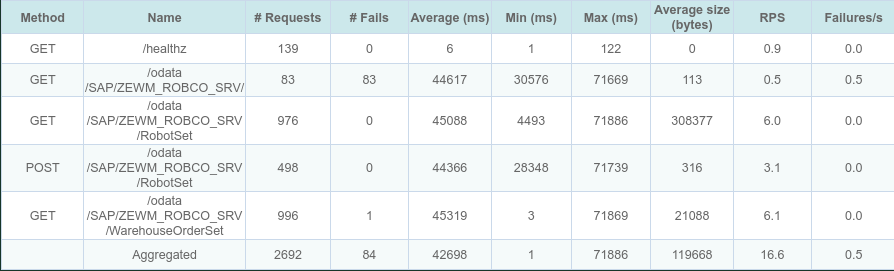
\includegraphics[width=\textwidth]{Bilder/perf-v1.png}
	\caption{Gemessene Performance der ersten Version des \ac{ewm-sim}}
	\label{fig:perf-v1}
\end{figure}

\begin{figure}[!ht]
	\centering
	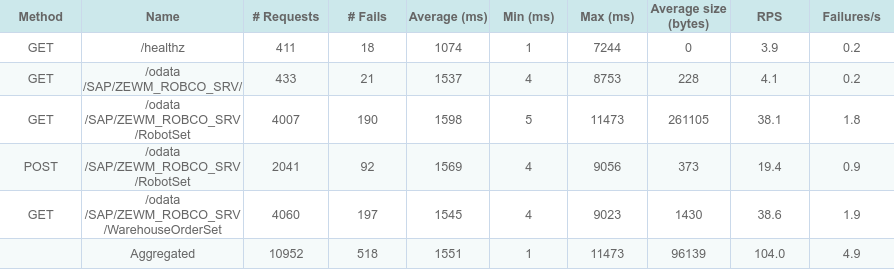
\includegraphics[width=\textwidth]{Bilder/perf-v2.png}
	\caption{Gemessene Performance der zweiten Version des \ac{ewm-sim}}
	\label{fig:perf-v2}
\end{figure}

\section{Future Work}
Trotz der nachweislich besseren Performance kam es bei der längeren Verwendung der neuen Version des \ac{ewm-sim} zu Probleme.
Diese bestehen darin, dass eine Funktionalität endlos neue Daten generiert.
Langfristig führt dies jedoch dazu, dass sich der Arbeitsspeicher viel zu stark ausgelastet wird, was schlussendlich zu einem Absturz des Simulators führen kann.

Zukünftig ist also auf jeden Fall dieser Missstand noch zu beheben.
Generell war im Rahmen dieser Projektarbeit keine Zeit für ausreichende Langzeittests oder eine Verknüpfung mit den Systemen, die später auf den \ac{ewm-sim} zurückgreifen sollen.
Diese Schritte müssen somit mit gebotener Sorgfalt durchgeführt werden, um auch langfristig einen reibungslosen Betrieb zu gewährleisten.

Des Weiteren wird momentan mit node-ui5 auf ein nicht aktiv entwickeltes und gepflegtes Produkt zurückgegriffen, welches überdies die Komponenten von SAPUI5 in einer Art und Weise verwendet, welche von SAP nie vorgesehen war.
Die aktuelle Implementierung auf Basis von node-ui5 eignet sich zwar schon deutlich besser, als die ursprüngliche, welche innerhalb eines headless Browsers lief, jedoch ist weiterhin ein Overhead vorhandenen.
Aus diesen Gründen sollte es langfristig in Betracht gezogen werden, die node-ui5-Basis durch eine eigene OData-Implementierung zu ersetzen.

Allerdings muss bei alldem auch betrachtet werden, dass es sich bei dem \ac{ewm-sim} eben um eine Simulationsumgebung handelt und nicht um ein Produktivsystem.
High Level Performance ist somit nicht kritisch und aufgrund des erheblichen Arbeitsaufwands, welcher mit den vorgeschlagenen Verbesserungen verbunden ist, ist die Umsetzung der meisten davon vermutlich nicht sinnvoll.

Der vollständige Quellcode des Projekts kann unter \url{https://github.com/SAP/ewm-cloud-robotics/tree/0353baf3532041cecffcc4243ae52d78a467d5cf/docker/ewm-sim} (Abgabezeitpunkt) und \url{https://github.com/SAP/ewm-cloud-robotics/tree/master/docker/ewm-sim} (aktueller Entwicklungsstand) eingesehen werden.